% !TeX program = xelatex
\documentclass[10pt]{article}
\usepackage[a3paper,portrait,margin=11mm]{geometry}
\usepackage{amsmath,amssymb,bm,graphicx,booktabs,array,xcolor}
\usepackage{newtxtext,newtxmath}
\usepackage{microtype}
\usepackage{fix-cm}
\usepackage[colorlinks=true,urlcolor=teal]{hyperref}
\definecolor{navy}{HTML}{152C46}
\definecolor{teal}{HTML}{007C83}
\definecolor{muted}{HTML}{526171}
\definecolor{pale}{HTML}{EAF4F3}
\definecolor{line}{HTML}{CFD8E0}
\pagestyle{empty}
\linespread{1.0}
\setlength{\parindent}{0pt}
\setlength{\parskip}{2pt}
\setlength{\abovedisplayskip}{2pt}
\setlength{\belowdisplayskip}{2pt}
\setlength{\abovedisplayshortskip}{2pt}
\setlength{\belowdisplayshortskip}{2pt}
\newcommand{\sect}[2]{\par\vspace{2pt}{\color{teal}\bfseries\fontsize{13.5}{16}\selectfont #1\quad #2}\par\vspace{1pt}{\color{line}\hrule}\vspace{2pt}}
\newcommand{\subhead}[1]{\par\vspace{2pt}{\bfseries\color{navy}#1}\par}
\newcommand{\smallnote}[1]{{\fontsize{8.6}{10.7}\selectfont\color{muted}#1\par}}
\newcommand{\takeaway}[1]{\par\vspace{3pt}\colorbox{pale}{\parbox{\dimexpr\linewidth-2\fboxsep}{\bfseries\color{teal}#1}}\par}
\newcommand{\posterheader}[3]{\colorbox{navy}{\parbox{\dimexpr\textwidth-2\fboxsep}{\vspace{5mm}\hspace{3mm}\begin{minipage}{\dimexpr\linewidth-6mm}\color{white}{\bfseries\fontsize{24}{27}\selectfont #1\par}\vspace{2mm}{\fontsize{11}{14}\selectfont #2\hfill #3}\end{minipage}\vspace{5mm}}}\par\vspace{4mm}}
\newcommand{\columnstart}{\begin{minipage}[t]{0.318\textwidth}\vspace{0pt}}
\newcommand{\columnend}{\end{minipage}}
\newcommand{\colsep}{\hfill}
\newcommand{\posterfooter}[1]{\par\vspace{3mm}{\color{line}\hrule}\vspace{1.5mm}{\fontsize{8}{10}\selectfont\color{muted}#1\par}}

\newcommand{\extrablock}[1]{\par\vspace{5pt}{\color{teal}\bfseries\fontsize{12}{15}\selectfont #1}\par\vspace{2pt}}

\begin{document}
\fontsize{10.3}{12.7}\selectfont
\posterheader{Variable-Thrust, Variable-Mass Rockets:\\Near-Earth Flight and Control}{Chengguo Jin · Taorui Zhang · Shiji Jiang · Zhaoyuan Zhang}{Applied Mathematical Methods | 2026}
\columnstart
\sect{01}{Problem \& physical model}
\textbf{Orbit insertion requires both altitude and velocity.} Near-Earth orbits enable observation, space experiments and subsequent missions. Reaching altitude without sufficient transverse speed yields a suborbital return.
\subhead{Vertical ascent and ideal propulsion}
For expelled mass $-\mathrm dm>0$ and relative exhaust speed $v_e$ (also denoted by $c$ below), momentum balance gives
\[
 m\,\mathrm dv=-v_e\,\mathrm dm+F_{\rm ext}\,\mathrm dt.
\]
Neglecting external forces and integrating yields the Tsiolkovsky equation:
\[
 \boxed{\Delta v_{\rm ideal}=c\ln(m_0/m_f)}.
\]
Impulse is $I_T=\int T\,\mathrm dt=v_e(m_0-m_f)$; velocity gain integrates $T/m$. Starting from rest with $r\ge r_0$, no random forcing and dissipative drag, ideal propulsion and orbital energy imply
\[
 \frac{m_0}{m_f}\ge\exp\!\left[\frac{\sqrt{2\mu/r_0-\mu/r_*}}{v_e}\right].
\]
The necessary mass ratio is at least \textbf{6.245} in the 600 km case; this bound is not sufficient for insertion.
\subhead{Earth-centered planar polar dynamics}
Define $u=\dot r$, $w=r\dot\theta$, $V=\sqrt{u^2+w^2}$, propellant flow $q=-\dot m\ge0$ and thrust $T=cq$.
\[
\begin{aligned}
 \dot r&=u,\qquad \dot\theta=w/r,\qquad \dot m=-q,\\
 \dot u&=\frac{w^2}{r}+\frac{cq\cos\alpha}{m}-\frac{\mu}{r^2}
 -\frac{kVu}{m}+a_{\varepsilon,r},\\
 \dot w&=-\frac{uw}{r}+\frac{cq\sin\alpha}{m}
 -\frac{kVw}{m}+a_{\varepsilon,\theta}.
\end{aligned}
\]
Here $k=\rho C_DA/2$ and $\rho=\rho_0e^{-(r-R_E)/H}$. Thrust follows $\alpha=\operatorname{atan2}(w,u)+\delta$ after a short initial vertical hold.
\[
 a_{\varepsilon,j}=\sigma_{0,j}(\rho/\rho_{\rm ref})\eta_j(t).
\]
\smallnote{Gaussian forcing is continuously interpolated with finite temporal correlation, not ideal white noise. The planar point-mass model omits Earth rotation, lift and attitude actuator dynamics.}

\extrablock{Physical settings and capability}
{\fontsize{9.2}{12}\selectfont
\begin{tabular*}{\linewidth}{@{\extracolsep{\fill}}lr@{}}\toprule
Initial / dry mass & $60\,000 / 1\,200$ kg\\
Effective exhaust speed & $4\,500$ m/s\\
Drag coefficient / area & $0.35 / 2.0$ m$^2$\\
Density / scale height & $1.225$ kg/m$^3$ / $8.5$ km\\
Disturbance at reference density & $0.1$ m/s$^2$\\\bottomrule
\end{tabular*}}
Circular speed is about $7.562$ km/s; the energy-based ideal velocity bound is $8.243$ km/s. The achieved mass ratio is $9.636$, above the necessary bound, reflecting finite thrust, steering and external-force losses.
\extrablock{Numerical integration links control to flight}
For $\dot y=f(t,y)$, classical RK4 evaluates four slopes:
\[
 y_{n+1}=y_n+\frac{\Delta t}{6}(K_1+2K_2+2K_3+K_4).
\]
Batched GPU RK4 can also accelerate simulation and substantially reduce computation time.
\takeaway{The mass-ratio lower bound from Tsiolkovsky's equation guides initialization and feasibility screening for ODE-based trajectory optimization.}

\columnend\colsep
\columnstart
\sect{02}{Planning \& feedback control}
\subhead{Trajectory planning: PSO search with SQP refinement}
A suborbital burn, coast and circularization burn structure the search over thrust-angle nodes, flow rates and phase durations. PSO combines personal and neighborhood experience; SQP then refines terminal feasibility.
\[
 r_*=R_E+600\,\mathrm{km},\qquad v_c=\sqrt{\mu/r_*},
\]
\[
 J=\left(\frac{r_f-r_*}{s_h}\right)^2+
 \left(\frac{u_f}{s_u}\right)^2+
 \left(\frac{w_f-v_c}{s_w}\right)^2.
\]

\subhead{How PSO works}
In normalized design space, particle position and search velocity are $\xi_i,\nu_i$; personal and neighborhood bests are $p_i,g_i$:
\[
\begin{aligned}
 \nu_i^{k+1}&=\omega\nu_i^k+c_1r_1\odot(p_i-\xi_i^k)\\
 &\quad+c_2r_2\odot(g_i-\xi_i^k),\\
 \xi_i^{k+1}&=\xi_i^k+\nu_i^{k+1}.
\end{aligned}
\]
Random exploration and shared experience reduce terminal error. Bounds, impact and propellant-budget violations are constrained or penalized. PSO does not guarantee a global optimum; fuel minimization is not the objective here.

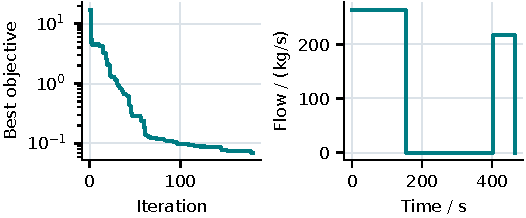
\includegraphics[width=\linewidth,height=42mm]{images/planning_en.pdf}
\smallnote{Left: PSO objective history. Right: final reference flow. Burn/coast/burn durations are approximately 153.3 / 250.0 / 62.0 s. Final accuracy reflects both PSO and local refinement.}
\subhead{MPC: measure, predict, solve, apply}
Track $x^{\rm ref}=(r,\theta,u,w,m)^\mathsf T$ using thrust-angle and flow corrections. Linearizing the discrete dynamics along the reference gives
\[
 e_{k+1}=A_ke_k+B_kv_k+d_k.
\]

\subhead{Receding-horizon cost and constraints}
\[
\begin{aligned}
 J_{\rm MPC}={}&\sum_{j=1}^{N}\|e_{k+j|k}\|_{Q_j}^2
 +\sum_{j=0}^{N-1}\|v_{k+j|k}\|_R^2\\
 &+\sum_{j=0}^{N-1}\|\Delta v_{k+j|k}\|_{R_\Delta}^2
 +\lambda\|\epsilon\|^2.
\end{aligned}
\]
The tracking error $e$ and control correction $v$ are normalized by physical scales. Ground clearance is softened; dry-mass and input limits are enforced as hard constraints.

Quadratic penalties on predicted tracking errors, control effort, control changes and slack variables are condensed into a convex quadratic program:
\[
 \min_\zeta\ \tfrac12\zeta^\mathsf TH\zeta+f^\mathsf T\zeta,
 \qquad G\zeta\le b.
\]
A \textbf{convex interior-point algorithm} solves the QP with angle, flow, dry-mass and ground constraints. Apply only the first correction, then repeat with fresh state feedback; retain the two-burn schedule.

\subhead{Why is the QP convex?}
After state elimination, $H=2(\mathcal B^\mathsf T\bar Q\mathcal B+\bar R+D^\mathsf T\bar R_\Delta D)$. Positive-definite input weighting makes $H$ positive definite. The interior-point solver follows perturbed KKT conditions as the barrier parameter decreases.

\takeaway{Offline planning supplies a feasible reference; online MPC corrects disturbances in flight.}
\columnend\colsep
\columnstart
\sect{03}{600 km case \& findings}
\smallnote{$m_0=60\,000$ kg, $m_{\rm dry}=1\,200$ kg, $c=4\,500$ m/s. Open and closed loops share the same plant disturbance, distinct from the planning realization.}
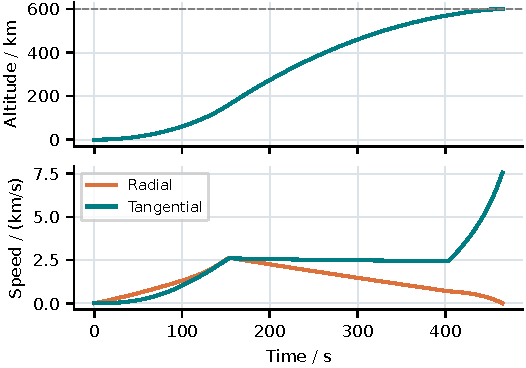
\includegraphics[width=\linewidth,height=60mm]{images/reference_en.pdf}
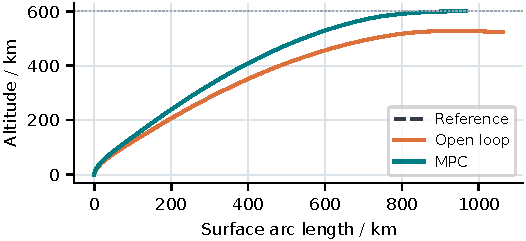
\includegraphics[width=\linewidth,height=48mm]{images/trajectory_en.pdf}
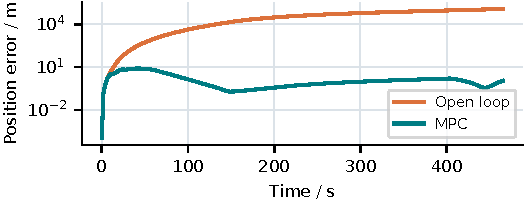
\includegraphics[width=\linewidth,height=40mm]{images/error_en.pdf}
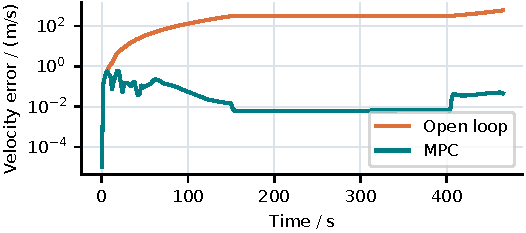
\includegraphics[width=\linewidth,height=40mm]{images/velocity_en.pdf}
\smallnote{MPC nearly overlaps the reference trajectory. Position error combines radial and surface-arc errors; zero values are floored only for logarithmic plotting.}
\vspace{2pt}
{\fontsize{9.2}{12}\selectfont
\setlength{\tabcolsep}{2pt}
\begin{tabular*}{\linewidth}{@{\extracolsep{\fill}}lrr@{}}
\toprule
Metric & Open loop & MPC\\\midrule
Position RMS / m & $5.98\times10^4$ & $2.606$\\
Velocity RMS / (m/s) & $298.084$ & $0.0992$\\
Cutoff altitude error / m & $-77\,611.6$ & $1.191$\\
Cutoff radial speed / (m/s) & $-557.983$ & $0.0231$\\
Tangential speed error / (m/s) & $233.256$ & $0.0559$\\\bottomrule
\end{tabular*}}
\smallnote{RMS is relative to the reference; cutoff errors are relative to the target circular orbit.}
\extrablock{Flight phases and online computation}
The first burn builds ascent and transverse motion; coasting gains altitude; the second burn raises transverse speed and reduces radial speed. Reference cutoff residuals are $0.265$ m, $-0.0212$ m/s and $0.0463$ m/s.
MPC updates every 2 s with a 30 s horizon. All 230 QPs succeeded; mean solve time was 1.793 ms.

\takeaway{Feedback suppresses error accumulation and brings cutoff close to circular-orbit conditions.}
\columnend
\posterfooter{References: NASA Glenn, Ideal Rocket Equation; Kennedy \& Eberhart, Particle Swarm Optimization, 1995; Dormand \& Prince, JCAM, 1980; Mayne et al., Automatica, 2000; Nocedal \& Wright, Numerical Optimization, 2006.\quad Data: project experiment snapshot, 20 Oct 2026.}
\end{document}
